\documentclass{article}
\usepackage{import}
\import{../../lib/latex/}{wgmlgz}
\begin{document}

\itmo[
  variant=161,
  labn=4,
  worktype=Домашняя работа,
  discipline=Дискретная математика,
  group=P3115,
  student=Владимир Мацюк,
  teacher=Поляков Владимир Иванович,
  logo=../../lib/img/itmo.png
]





Исходная таблица соединений R:



$$\begin{tabular}{|c|c|c|c|c|c|c|c|c|c|c|c|c|c|c|c|c|c|c|c|c|c|c|c|} \hline

    v/v & e1 & e2 & e3 & e4 & e5 & e6 & e7 & e8 & e9 & e10 & e11 & e12 \nl

    e1  & 0  & 3  &    &    & 4  & 4  & 4  & 4  &    & 3   & 4   & \nl

    e2  & 3  & 0  & 1  &    &    &    &    & 4  &    & 2   &     & \nl

    e3  &    & 1  & 0  & 5  &    &    &    &    & 3  & 1   &     & \nl

    e4  &    &    & 5  & 0  & 1  & 4  & 1  &    & 4  & 5   & 4   & \nl

    e5  & 4  &    &    & 1  & 0  & 1  &    &    &    & 3   &     & \nl

    e6  & 4  &    &    & 4  & 1  & 0  & 2  &    &    &     & 4   & \nl

    e7  & 4  &    &    & 1  &    & 2  & 0  &    &    & 4   &     & 1 \nl

    e8  & 4  & 4  &    &    &    &    &    & 0  & 3  & 3   &     & 5 \nl

    e9  &    &    & 3  & 4  &    &    &    & 3  & 0  &     & 5   & \nl

    e10 & 3  & 2  & 1  & 5  & 3  &    & 4  & 3  &    & 0   & 2   & \nl

    e11 & 4  &    &    & 4  &    & 4  &    &    & 8  & 2   & 0   & 4 \nl

    e12 &    &    &    &    &    &    & 1  & 5  &    &     & 4   & 0\nl
  \end{tabular}$$









\section{Найти гамильтонов цикл}



Включаем в S вершину x1. S=\{x1\}



Возможная вершина: x2. S=\{x1,x2\}



Возможная вершина: x3. S=\{x1,x2,x3\}



Возможная вершина: x4. S=\{x1,x2,x3,x4\}



Возможная вершина: x5. S=\{x1,x2,x3,x4,x5\}



Возможная вершина: x6. S=\{x1,x2,x3,x4,x5,x6\}



Возможная вершина: x7. S=\{x1,x2,x3,x4,x5,x6,x7\}



Возможная вершина: x10. S=\{x1,x2,x3,x4,x5,x6,x7,x10\}



Возможная вершина: x8. S=\{x1,x2,x3,x4,x5,x6,x7,x10,x8\}



Возможная вершина: x9. S=\{x1,x2,x3,x4,x5,x6,x7,x10,x8,x9\}



Возможная вершина: x11. S=\{x1,x2,x3,x4,x5,x6,x7,x10,x8,x9,x11\}



Возможная вершина: x12. S=\{x1,x2,x3,x4,x5,x6,x7,x10,x8,x9,x11,x12\}



Ребра (x12,x1) нет, найдена гамильтонова цепь. Прибегнем к возвращению: удалим из S вершину x12, перейдем к x11. S=\{x1,x2,x3,x4,x5,x6,x7,x10,x8,x9,x11\}



У x11 больше нет возможных вершин, удалим ее. Перейдем к x9. S=\{x1,x2,x3,x4,x5,x6,x7,x10,x8,x9\}



У x9 больше нет возможных вершин, удалим ее. Перейдем к x8. S=\{x1,x2,x3,x4,x5,x6,x7,x10,x8\}



Возможная вершина: x12. S=\{x1,x2,x3,x4,x5,x6,x7,x10,x8,x12\}



Возможная вершина: x11. S=\{x1,x2,x3,x4,x5,x6,x7,x10,x8,x12,x11\}



Возможная вершина: x9. S=\{x1,x2,x3,x4,x5,x6,x7,x10,x8,x12,x11,x9\}



Ребра (x9,x1) нет, найдена гамильтонова цепь. Прибегнем к возвращению: удалим из S вершину x9, перейдем к x11. S=\{x1,x2,x3,x4,x5,x6,x7,x10,x8,x12,x11\}



У x11 больше нет возможных вершин, удалим ее. Перейдем к x12. S=\{x1,x2,x3,x4,x5,x6,x7,x10,x8,x12\}



У x12 больше нет возможных вершин, удалим ее. Перейдем к x8. S=\{x1,x2,x3,x4,x5,x6,x7,x10,x8\}



У x8 больше нет возможных вершин, удалим ее. Перейдем к x10. S=\{x1,x2,x3,x4,x5,x6,x7,x10\}



Возможная вершина: x11. S=\{x1,x2,x3,x4,x5,x6,x7,x10,x11\}



Возможная вершина: x9. S=\{x1,x2,x3,x4,x5,x6,x7,x10,x11,x9\}



Возможная вершина: x8. S=\{x1,x2,x3,x4,x5,x6,x7,x10,x11,x9,x8\}



Возможная вершина: x12. S=\{x1,x2,x3,x4,x5,x6,x7,x10,x11,x9,x8,x12\}



Ребра (x12,x1) нет, найдена гамильтонова цепь. Прибегнем к возвращению: удалим из S вершину x12, перейдем к x8. S=\{x1,x2,x3,x4,x5,x6,x7,x10,x11,x9,x8\}



У x8 больше нет возможных вершин, удалим ее. Перейдем к x9. S=\{x1,x2,x3,x4,x5,x6,x7,x10,x11,x9\}



У x9 больше нет возможных вершин, удалим ее. Перейдем к x11. S=\{x1,x2,x3,x4,x5,x6,x7,x10,x11\}



Возможная вершина: x12. S=\{x1,x2,x3,x4,x5,x6,x7,x10,x11,x12\}



Возможная вершина: x8. S=\{x1,x2,x3,x4,x5,x6,x7,x10,x11,x12,x8\}



Возможная вершина: x9. S=\{x1,x2,x3,x4,x5,x6,x7,x10,x11,x12,x8,x9\}



Ребра (x9,x1) нет, найдена гамильтонова цепь. Прибегнем к возвращению: удалим из S вершину x9, перейдем к x8. S=\{x1,x2,x3,x4,x5,x6,x7,x10,x11,x12,x8\}



У x8 больше нет возможных вершин, удалим ее. Перейдем к x12. S=\{x1,x2,x3,x4,x5,x6,x7,x10,x11,x12\}



У x12 больше нет возможных вершин, удалим ее. Перейдем к x11. S=\{x1,x2,x3,x4,x5,x6,x7,x10,x11\}



У x11 больше нет возможных вершин, удалим ее. Перейдем к x10. S=\{x1,x2,x3,x4,x5,x6,x7,x10\}



У x10 больше нет возможных вершин, удалим ее. Перейдем к x7. S=\{x1,x2,x3,x4,x5,x6,x7\}



Возможная вершина: x12. S=\{x1,x2,x3,x4,x5,x6,x7,x12\}



Возможная вершина: x8. S=\{x1,x2,x3,x4,x5,x6,x7,x12,x8\}



Возможная вершина: x9. S=\{x1,x2,x3,x4,x5,x6,x7,x12,x8,x9\}



Возможная вершина: x11. S=\{x1,x2,x3,x4,x5,x6,x7,x12,x8,x9,x11\}



Возможная вершина: x10. S=\{x1,x2,x3,x4,x5,x6,x7,x12,x8,x9,x11,x10\}



Гамильтонов цикл найден. S=\{x1,x2,x3,x4,x5,x6,x7,x12,x8,x9,x11,x10\}






\begin{center}

  Матрица смежности с перенумерованными вершинами

  \begin{tabular}{|c|c|c|c|c|c|c|c|c|c|c|c|c|} \hline

    0 & 1 & 0 & 0 & 1 & 1 & 1 & 0 & 1 & 0 & 1 & 1\nl

    1 & 0 & 1 & 0 & 0 & 0 & 0 & 0 & 1 & 0 & 0 & 1\nl

    0 & 1 & 0 & 1 & 0 & 0 & 0 & 0 & 0 & 1 & 0 & 1\nl

    0 & 0 & 1 & 0 & 1 & 1 & 1 & 0 & 0 & 1 & 1 & 1\nl

    1 & 0 & 0 & 1 & 0 & 1 & 0 & 0 & 0 & 0 & 0 & 1\nl

    1 & 0 & 0 & 1 & 1 & 0 & 1 & 0 & 0 & 0 & 1 & 0\nl

    1 & 0 & 0 & 1 & 0 & 1 & 0 & 1 & 0 & 0 & 0 & 1\nl

    0 & 0 & 0 & 0 & 0 & 0 & 1 & 0 & 1 & 0 & 1 & 0\nl

    1 & 1 & 0 & 0 & 0 & 0 & 0 & 1 & 0 & 1 & 0 & 1\nl

    0 & 0 & 1 & 1 & 0 & 0 & 0 & 0 & 1 & 0 & 1 & 0\nl

    1 & 0 & 0 & 1 & 0 & 1 & 0 & 1 & 0 & 1 & 0 & 1\nl

    1 & 1 & 1 & 1 & 1 & 0 & 1 & 0 & 1 & 0 & 1 & 0\nl
  \end{tabular}

\end{center}



\begin{itemize}
  \item до перенумерации	  x1	x2	x3	x4	x5	x6	x7	x12	x8	x9	x11	x10
  \item после перенумерации	x1	x2	x3	x4	x5	x6	x7	x8	x9	x10	x11	x12
\end{itemize}



\section{Построение графа пересечений G'}



Определим p212, для чего в матрице R выделим подматрицу R212.



Ребро (x2x12) пересекается с (x1x5),(x1x6),(x1x7),(x1x9),(x1x11)



Определим p29, для чего в матрице R выделим подматрицу R29.



Ребро (x2x9) пересекается с (x1x5),(x1x6),(x1x7)



Определим p312, для чего в матрице R выделим подматрицу R312.



Ребро (x3x12) пересекается с (x1x5),(x1x6),(x1x7),(x1x9),(x1x11),(x2x9)



Определим p310, для чего в матрице R выделим подматрицу R310.



Ребро (x3x10) пересекается с (x1x5),(x1x6),(x1x7),(x1x9),(x2x9)



Определим p412, для чего в матрице R выделим подматрицу R412.



Ребро (x4x12) пересекается с (x1x5),(x1x6),(x1x7),(x1x9),(x1x11),(x2x9),(x3x10)



Определим p411, для чего в матрице R выделим подматрицу R411.



Ребро (x4x11) пересекается с (x1x5),(x1x6),(x1x7),(x1x9),(x2x9),(x3x10)



Определим p410, для чего в матрице R выделим подматрицу R410.



Ребро (x4x10) пересекается с (x1x5),(x1x6),(x1x7),(x1x9),(x2x9)



Определим p47, для чего в матрице R выделим подматрицу R47.



Ребро (x4x7) пересекается с (x1x5),(x1x6)



Определим p46, для чего в матрице R выделим подматрицу R46.



Ребро (x4x6) пересекается с (x1x5)



Определим p512, для чего в матрице R выделим подматрицу R512.



Ребро (x5x12) пересекается с (x1x6),(x1x7),(x1x9),(x1x11),(x2x9),(x3x10),(x4x6),(x4x7),(x4x10),(x4x11)



15 пересечений графа найдено, закончим поиск.







\begin{tabular}{|c|c|c|c|c|c|c|c|c|c|c|c|c|c|c|c|c|c|c|c|c|c|c|c|c|c|c|} \hline

               & $p_{1\ 5} $ & $p_{2\ 12} $ & $p_{1\ 6} $ & $p_{1\ 7} $ & $p_{1\ 9} $ & $p_{1\ 11} $ & $p_{2\ 9} $ & $p_{3\ 12} $ & $p_{3\ 10} $ & $p_{4\ 12} $ & $p_{4\ 11} $ & $p_{4\ 10} $ & $p_{4\ 7} $ & $p_{4\ 6} $ & $p_{5\ 12}$ \nl

  $p_{1\ 5} $  & 1           & 1            & 0           & 0           & 0           & 0            & 1           & 1            & 1            & 1            & 1            & 1            & 1           & 1           & 0 \nl

  $p_{2\ 12} $ & 1           & 1            & 1           & 1           & 1           & 1            & 0           & 0            & 0            & 0            & 0            & 0            & 0           & 0           & 0 \nl

  $p_{1\ 6} $  & 0           & 1            & 1           & 0           & 0           & 0            & 1           & 1            & 1            & 1            & 1            & 1            & 1           & 0           & 1 \nl

  $p_{1\ 7} $  & 0           & 1            & 0           & 1           & 0           & 0            & 1           & 1            & 1            & 1            & 1            & 1            & 0           & 0           & 1 \nl

  $p_{1\ 9} $  & 0           & 1            & 0           & 0           & 1           & 0            & 0           & 1            & 1            & 1            & 1            & 1            & 0           & 0           & 1 \nl

  $p_{1\ 11} $ & 0           & 1            & 0           & 0           & 0           & 1            & 0           & 1            & 0            & 1            & 0            & 0            & 0           & 0           & 1 \nl

  $p_{2\ 9} $  & 1           & 0            & 1           & 1           & 0           & 0            & 1           & 1            & 1            & 1            & 1            & 1            & 0           & 0           & 1 \nl

  $p_{3\ 12} $ & 1           & 0            & 1           & 1           & 1           & 1            & 1           & 1            & 0            & 0            & 0            & 0            & 0           & 0           & 0 \nl

  $p_{3\ 10} $ & 1           & 0            & 1           & 1           & 1           & 0            & 1           & 0            & 1            & 1            & 1            & 0            & 0           & 0           & 1 \nl

  $p_{4\ 12} $ & 1           & 0            & 1           & 1           & 1           & 1            & 1           & 0            & 1            & 1            & 0            & 0            & 0           & 0           & 0 \nl

  $p_{4\ 11} $ & 1           & 0            & 1           & 1           & 1           & 0            & 1           & 0            & 1            & 0            & 1            & 0            & 0           & 0           & 1 \nl

  $p_{4\ 10} $ & 1           & 0            & 1           & 1           & 1           & 0            & 1           & 0            & 0            & 0            & 0            & 1            & 0           & 0           & 1 \nl

  $p_{4\ 7} $  & 1           & 0            & 1           & 0           & 0           & 0            & 0           & 0            & 0            & 0            & 0            & 0            & 1           & 0           & 1 \nl

  $p_{4\ 6} $  & 1           & 0            & 0           & 0           & 0           & 0            & 0           & 0            & 0            & 0            & 0            & 0            & 0           & 1           & 1 \nl

  $p_{5\ 12} $ & 0           & 0            & 1           & 1           & 1           & 1            & 1           & 0            & 1            & 0            & 1            & 1            & 1           & 1           & 1 \nl
\end{tabular}



\section{Построение семейства ψG}



В 1 строке ищем первый нулевой элемент - $r_{1\ 3}$.

Записываем дизъюнкцию $M_{1\ 3} = r_{1}\lor r_{3} = 110000111111110 \lor 011000111111101 = 111000111111111$

В строке $M_{1\ 3}$ находим номера нулевых элементов, составляем список $J' = \{4, 5, 6\}$.

Записываем дизъюнкцию $M_{1\ 3\ 4} = M_{1\ 3}\lor r_{4} = 111000111111111 \lor 010100111111001 = 111100111111111$

В строке $M_{1\ 3\ 4}$ находим номера нулевых элементов, составляем список $J' = \{5, 6\}$.

Записываем дизъюнкцию $M_{1\ 3\ 4\ 5} = M_{1\ 3\ 4}\lor r_{5} = 111100111111111 \lor 010010011111001 = 111110111111111$

В строке $M_{1\ 3\ 4\ 5}$ находим номера нулевых элементов, составляем список $J' = \{6\}$.

Записываем дизъюнкцию $M_{1\ 3\ 4\ 5\ 6} = M_{1\ 3\ 4\ 5}\lor r_{6} = 111110111111111 \lor 010001010100001 = 111111111111111$

В строке $M_{1\ 3\ 4\ 5\ 6}$ все 1. Построено $\psi_{1} = \{u_{1\ 5},u_{1\ 6},u_{1\ 7},u_{1\ 9},u_{1\ 11}\}$

Записываем дизъюнкцию $M_{1\ 3\ 4\ 6} = M_{1\ 3\ 4}\lor r_{6} = 111100111111111 \lor 010001010100001 = 111101111111111$

В строке $M_{1\ 3\ 4\ 6}$ остались незакрытые 0.

Записываем дизъюнкцию $M_{1\ 3\ 5} = M_{1\ 3}\lor r_{5} = 111000111111111 \lor 010010011111001 = 111010111111111$

В строке $M_{1\ 3\ 5}$ находим номера нулевых элементов, составляем список $J' = \{6\}$.

Строка 6 не закроет ноль на 4 позиции.

Записываем дизъюнкцию $M_{1\ 3\ 6} = M_{1\ 3}\lor r_{6} = 111000111111111 \lor 010001010100001 = 111001111111111$

В строке $M_{1\ 3\ 6}$ остались незакрытые 0.

Записываем дизъюнкцию $M_{1\ 4} = r_{1}\lor r_{4} = 110000111111110 \lor 010100111111001 = 110100111111111$

В строке $M_{1\ 4}$ находим номера нулевых элементов, составляем список $J' = \{5, 6\}$.

Строки 5, 6 не закроют ноль на 3 позиции.

Записываем дизъюнкцию $M_{1\ 5} = r_{1}\lor r_{5} = 110000111111110 \lor 010010011111001 = 110010111111111$

В строке $M_{1\ 5}$ находим номера нулевых элементов, составляем список $J' = \{6\}$.

Строка 6 не закроет нули на позициях 3, 4

Записываем дизъюнкцию $M_{1\ 6} = r_{1}\lor r_{6} = 110000111111110 \lor 010001010100001 = 110001111111111$

В строке $M_{1\ 6}$ остались незакрытые 0.

Записываем дизъюнкцию $M_{1\ 15} = r_{1}\lor r_{15} = 110000111111110 \lor 001111101011111 = 111111111111111$

В строке $M_{1\ 15}$ все 1. Построено $\psi_{2} = \{u_{1\ 5},u_{5\ 12}\}$



В 2 строке ищем первый нулевой элемент - $r_{2\ 7}$.

Записываем дизъюнкцию $M_{2\ 7} = r_{2}\lor r_{7} = 111111000000000 \lor 101100111111001 = 111111111111001$

В строке $M_{2\ 7}$ находим номера нулевых элементов, составляем список $J' = \{13, 14\}$.

Записываем дизъюнкцию $M_{2\ 7\ 13} = M_{2\ 7}\lor r_{13} = 111111111111001 \lor 101000000000101 = 111111111111101$

В строке $M_{2\ 7\ 13}$ находим номера нулевых элементов, составляем список $J' = \{14\}$.

Записываем дизъюнкцию $M_{2\ 7\ 13\ 14} = M_{2\ 7\ 13}\lor r_{14} = 111111111111101 \lor 100000000000011 = 111111111111111$

В строке $M_{2\ 7\ 13\ 14}$ все 1. Построено $\psi_{3} = \{u_{2\ 12},u_{2\ 9},u_{4\ 7},u_{4\ 6}\}$

Записываем дизъюнкцию $M_{2\ 7\ 14} = M_{2\ 7}\lor r_{14} = 111111111111001 \lor 100000000000011 = 111111111111011$

В строке $M_{2\ 7\ 14}$ остались незакрытые 0.

Записываем дизъюнкцию $M_{2\ 8} = r_{2}\lor r_{8} = 111111000000000 \lor 101111110000000 = 111111110000000$

В строке $M_{2\ 8}$ находим номера нулевых элементов, составляем список $J' = \{9, 10, 11, 12, 13, 14, 15\}$.

Записываем дизъюнкцию $M_{2\ 8\ 9} = M_{2\ 8}\lor r_{9} = 111111110000000 \lor 101110101110001 = 111111111110001$

В строке $M_{2\ 8\ 9}$ находим номера нулевых элементов, составляем список $J' = \{12, 13, 14\}$.

Записываем дизъюнкцию $M_{2\ 8\ 9\ 12} = M_{2\ 8\ 9}\lor r_{12} = 111111111110001 \lor 101110100001001 = 111111111111001$

В строке $M_{2\ 8\ 9\ 12}$ находим номера нулевых элементов, составляем список $J' = \{13, 14\}$.

Записываем дизъюнкцию $M_{2\ 8\ 9\ 12\ 13} = M_{2\ 8\ 9\ 12}\lor r_{13} = 111111111111001 \lor 101000000000101 = 111111111111101$

В строке $M_{2\ 8\ 9\ 12\ 13}$ находим номера нулевых элементов, составляем список $J' = \{14\}$.

Записываем дизъюнкцию $M_{2\ 8\ 9\ 12\ 13\ 14} = M_{2\ 8\ 9\ 12\ 13}\lor r_{14} = 111111111111101 \lor 100000000000011 = 111111111111111$

В строке $M_{2\ 8\ 9\ 12\ 13\ 14}$ все 1. Построено $\psi_{4} = \{u_{2\ 12},u_{3\ 12},u_{3\ 10},u_{4\ 10},u_{4\ 7},u_{4\ 6}\}$

Записываем дизъюнкцию $M_{2\ 8\ 9\ 12\ 14} = M_{2\ 8\ 9\ 12}\lor r_{14} = 111111111111001 \lor 100000000000011 = 111111111111011$

В строке $M_{2\ 8\ 9\ 12\ 14}$ остались незакрытые 0.

Записываем дизъюнкцию $M_{2\ 8\ 9\ 13} = M_{2\ 8\ 9}\lor r_{13} = 111111111110001 \lor 101000000000101 = 111111111110101$

В строке $M_{2\ 8\ 9\ 13}$ находим номера нулевых элементов, составляем список $J' = \{14\}$.

Строка 14 не закроет ноль на 12 позиции.

Записываем дизъюнкцию $M_{2\ 8\ 9\ 14} = M_{2\ 8\ 9}\lor r_{14} = 111111111110001 \lor 100000000000011 = 111111111110011$

В строке $M_{2\ 8\ 9\ 14}$ остались незакрытые 0.

Записываем дизъюнкцию $M_{2\ 8\ 10} = M_{2\ 8}\lor r_{10} = 111111110000000 \lor 101111101100000 = 111111111100000$

В строке $M_{2\ 8\ 10}$ находим номера нулевых элементов, составляем список $J' = \{11, 12, 13, 14, 15\}$.

Записываем дизъюнкцию $M_{2\ 8\ 10\ 11} = M_{2\ 8\ 10}\lor r_{11} = 111111111100000 \lor 101110101010001 = 111111111110001$

В строке $M_{2\ 8\ 10\ 11}$ находим номера нулевых элементов, составляем список $J' = \{12, 13, 14\}$.

Записываем дизъюнкцию $M_{2\ 8\ 10\ 11\ 12} = M_{2\ 8\ 10\ 11}\lor r_{12} = 111111111110001 \lor 101110100001001 = 111111111111001$

В строке $M_{2\ 8\ 10\ 11\ 12}$ находим номера нулевых элементов, составляем список $J' = \{13, 14\}$.

Записываем дизъюнкцию $M_{2\ 8\ 10\ 11\ 12\ 13} = M_{2\ 8\ 10\ 11\ 12}\lor r_{13} = 111111111111001 \lor 101000000000101 = 111111111111101$

В строке $M_{2\ 8\ 10\ 11\ 12\ 13}$ находим номера нулевых элементов, составляем список $J' = \{14\}$.

Записываем дизъюнкцию $M_{2\ 8\ 10\ 11\ 12\ 13\ 14} = M_{2\ 8\ 10\ 11\ 12\ 13}\lor r_{14} = 111111111111101 \lor 100000000000011 = 111111111111111$

В строке $M_{2\ 8\ 10\ 11\ 12\ 13\ 14}$ все 1. Построено $\psi_{5} = \{u_{2\ 12},u_{3\ 12},u_{4\ 12},u_{4\ 11},u_{4\ 10},u_{4\ 7},u_{4\ 6}\}$

Записываем дизъюнкцию $M_{2\ 8\ 10\ 11\ 12\ 14} = M_{2\ 8\ 10\ 11\ 12}\lor r_{14} = 111111111111001 \lor 100000000000011 = 111111111111011$

В строке $M_{2\ 8\ 10\ 11\ 12\ 14}$ остались незакрытые 0.

Записываем дизъюнкцию $M_{2\ 8\ 10\ 11\ 13} = M_{2\ 8\ 10\ 11}\lor r_{13} = 111111111110001 \lor 101000000000101 = 111111111110101$

В строке $M_{2\ 8\ 10\ 11\ 13}$ находим номера нулевых элементов, составляем список $J' = \{14\}$.

Строка 14 не закроет ноль на 12 позиции.

Записываем дизъюнкцию $M_{2\ 8\ 10\ 11\ 14} = M_{2\ 8\ 10\ 11}\lor r_{14} = 111111111110001 \lor 100000000000011 = 111111111110011$

В строке $M_{2\ 8\ 10\ 11\ 14}$ остались незакрытые 0.

Записываем дизъюнкцию $M_{2\ 8\ 10\ 12} = M_{2\ 8\ 10}\lor r_{12} = 111111111100000 \lor 101110100001001 = 111111111101001$

В строке $M_{2\ 8\ 10\ 12}$ находим номера нулевых элементов, составляем список $J' = \{13, 14\}$.

Строки 13, 14 не закроют ноль на 11 позиции.

Записываем дизъюнкцию $M_{2\ 8\ 10\ 13} = M_{2\ 8\ 10}\lor r_{13} = 111111111100000 \lor 101000000000101 = 111111111100101$

В строке $M_{2\ 8\ 10\ 13}$ находим номера нулевых элементов, составляем список $J' = \{14\}$.

Строка 14 не закроет нули на позициях 11, 12

Записываем дизъюнкцию $M_{2\ 8\ 10\ 14} = M_{2\ 8\ 10}\lor r_{14} = 111111111100000 \lor 100000000000011 = 111111111100011$

В строке $M_{2\ 8\ 10\ 14}$ остались незакрытые 0.

Записываем дизъюнкцию $M_{2\ 8\ 10\ 15} = M_{2\ 8\ 10}\lor r_{15} = 111111111100000 \lor 001111101011111 = 111111111111111$

В строке $M_{2\ 8\ 10\ 15}$ все 1. Построено $\psi_{6} = \{u_{2\ 12},u_{3\ 12},u_{4\ 12},u_{5\ 12}\}$

Записываем дизъюнкцию $M_{2\ 8\ 11} = M_{2\ 8}\lor r_{11} = 111111110000000 \lor 101110101010001 = 111111111010001$

В строке $M_{2\ 8\ 11}$ находим номера нулевых элементов, составляем список $J' = \{12, 13, 14\}$.

Строки 12, 13, 14 не закроют ноль на 10 позиции.

Записываем дизъюнкцию $M_{2\ 8\ 12} = M_{2\ 8}\lor r_{12} = 111111110000000 \lor 101110100001001 = 111111110001001$

В строке $M_{2\ 8\ 12}$ находим номера нулевых элементов, составляем список $J' = \{13, 14\}$.

Строки 13, 14 не закроют нули на позициях 9, 10, 11

Записываем дизъюнкцию $M_{2\ 8\ 13} = M_{2\ 8}\lor r_{13} = 111111110000000 \lor 101000000000101 = 111111110000101$

В строке $M_{2\ 8\ 13}$ находим номера нулевых элементов, составляем список $J' = \{14\}$.

Строка 14 не закроет нули на позициях 9, 10, 11, 12

Записываем дизъюнкцию $M_{2\ 8\ 14} = M_{2\ 8}\lor r_{14} = 111111110000000 \lor 100000000000011 = 111111110000011$

В строке $M_{2\ 8\ 14}$ остались незакрытые 0.

Записываем дизъюнкцию $M_{2\ 8\ 15} = M_{2\ 8}\lor r_{15} = 111111110000000 \lor 001111101011111 = 111111111011111$

В строке $M_{2\ 8\ 15}$ остались незакрытые 0.

Записываем дизъюнкцию $M_{2\ 9} = r_{2}\lor r_{9} = 111111000000000 \lor 101110101110001 = 111111101110001$

В строке $M_{2\ 9}$ находим номера нулевых элементов, составляем список $J' = \{12, 13, 14\}$.

Строки 12, 13, 14 не закроют ноль на 8 позиции.

Записываем дизъюнкцию $M_{2\ 10} = r_{2}\lor r_{10} = 111111000000000 \lor 101111101100000 = 111111101100000$

В строке $M_{2\ 10}$ находим номера нулевых элементов, составляем список $J' = \{11, 12, 13, 14, 15\}$.

Строки 11, 12, 13, 14, 15 не закроют ноль на 8 позиции.

Записываем дизъюнкцию $M_{2\ 11} = r_{2}\lor r_{11} = 111111000000000 \lor 101110101010001 = 111111101010001$

В строке $M_{2\ 11}$ находим номера нулевых элементов, составляем список $J' = \{12, 13, 14\}$.

Строки 12, 13, 14 не закроют нули на позициях 8, 10

Записываем дизъюнкцию $M_{2\ 12} = r_{2}\lor r_{12} = 111111000000000 \lor 101110100001001 = 111111100001001$

В строке $M_{2\ 12}$ находим номера нулевых элементов, составляем список $J' = \{13, 14\}$.

Строки 13, 14 не закроют нули на позициях 8, 9, 10, 11

Записываем дизъюнкцию $M_{2\ 13} = r_{2}\lor r_{13} = 111111000000000 \lor 101000000000101 = 111111000000101$

В строке $M_{2\ 13}$ находим номера нулевых элементов, составляем список $J' = \{14\}$.

Строка 14 не закроет нули на позициях 7, 8, 9, 10, 11, 12

Записываем дизъюнкцию $M_{2\ 14} = r_{2}\lor r_{14} = 111111000000000 \lor 100000000000011 = 111111000000011$

В строке $M_{2\ 14}$ остались незакрытые 0.

Записываем дизъюнкцию $M_{2\ 15} = r_{2}\lor r_{15} = 111111000000000 \lor 001111101011111 = 111111101011111$

В строке $M_{2\ 15}$ остались незакрытые 0.



В 3 строке ищем первый нулевой элемент - $r_{3\ 4}$.

Записываем дизъюнкцию $M_{3\ 4} = r_{3}\lor r_{4} = 011000111111101 \lor 010100111111001 = 011100111111101$

В строке $M_{3\ 4}$ находим номера нулевых элементов, составляем список $J' = \{5, 6, 14\}$.

Записываем дизъюнкцию $M_{3\ 4\ 5} = M_{3\ 4}\lor r_{5} = 011100111111101 \lor 010010011111001 = 011110111111101$

В строке $M_{3\ 4\ 5}$ находим номера нулевых элементов, составляем список $J' = \{6, 14\}$.

Записываем дизъюнкцию $M_{3\ 4\ 5\ 6} = M_{3\ 4\ 5}\lor r_{6} = 011110111111101 \lor 010001010100001 = 011111111111101$

В строке $M_{3\ 4\ 5\ 6}$ находим номера нулевых элементов, составляем список $J' = \{14\}$.

Записываем дизъюнкцию $M_{3\ 4\ 5\ 6\ 14} = M_{3\ 4\ 5\ 6}\lor r_{14} = 011111111111101 \lor 100000000000011 = 111111111111111$

В строке $M_{3\ 4\ 5\ 6\ 14}$ все 1. Построено $\psi_{7} = \{u_{1\ 6},u_{1\ 7},u_{1\ 9},u_{1\ 11},u_{4\ 6}\}$

Записываем дизъюнкцию $M_{3\ 4\ 5\ 14} = M_{3\ 4\ 5}\lor r_{14} = 011110111111101 \lor 100000000000011 = 111110111111111$

В строке $M_{3\ 4\ 5\ 14}$ остались незакрытые 0.

Записываем дизъюнкцию $M_{3\ 4\ 6} = M_{3\ 4}\lor r_{6} = 011100111111101 \lor 010001010100001 = 011101111111101$

В строке $M_{3\ 4\ 6}$ находим номера нулевых элементов, составляем список $J' = \{14\}$.

Строка 14 не закроет ноль на 5 позиции.

Записываем дизъюнкцию $M_{3\ 4\ 14} = M_{3\ 4}\lor r_{14} = 011100111111101 \lor 100000000000011 = 111100111111111$

В строке $M_{3\ 4\ 14}$ остались незакрытые 0.

Записываем дизъюнкцию $M_{3\ 5} = r_{3}\lor r_{5} = 011000111111101 \lor 010010011111001 = 011010111111101$

В строке $M_{3\ 5}$ находим номера нулевых элементов, составляем список $J' = \{6, 14\}$.

Строки 6, 14 не закроют ноль на 4 позиции.

Записываем дизъюнкцию $M_{3\ 6} = r_{3}\lor r_{6} = 011000111111101 \lor 010001010100001 = 011001111111101$

В строке $M_{3\ 6}$ находим номера нулевых элементов, составляем список $J' = \{14\}$.

Строка 14 не закроет нули на позициях 4, 5

Записываем дизъюнкцию $M_{3\ 14} = r_{3}\lor r_{14} = 011000111111101 \lor 100000000000011 = 111000111111111$

В строке $M_{3\ 14}$ остались незакрытые 0.



В 4 строке ищем первый нулевой элемент - $r_{4\ 5}$.

Записываем дизъюнкцию $M_{4\ 5} = r_{4}\lor r_{5} = 010100111111001 \lor 010010011111001 = 010110111111001$

В строке $M_{4\ 5}$ находим номера нулевых элементов, составляем список $J' = \{6, 13, 14\}$.

Записываем дизъюнкцию $M_{4\ 5\ 6} = M_{4\ 5}\lor r_{6} = 010110111111001 \lor 010001010100001 = 010111111111001$

В строке $M_{4\ 5\ 6}$ находим номера нулевых элементов, составляем список $J' = \{13, 14\}$.

Записываем дизъюнкцию $M_{4\ 5\ 6\ 13} = M_{4\ 5\ 6}\lor r_{13} = 010111111111001 \lor 101000000000101 = 111111111111101$

В строке $M_{4\ 5\ 6\ 13}$ находим номера нулевых элементов, составляем список $J' = \{14\}$.

Записываем дизъюнкцию $M_{4\ 5\ 6\ 13\ 14} = M_{4\ 5\ 6\ 13}\lor r_{14} = 111111111111101 \lor 100000000000011 = 111111111111111$

В строке $M_{4\ 5\ 6\ 13\ 14}$ все 1. Построено $\psi_{8} = \{u_{1\ 7},u_{1\ 9},u_{1\ 11},u_{4\ 7},u_{4\ 6}\}$

Записываем дизъюнкцию $M_{4\ 5\ 6\ 14} = M_{4\ 5\ 6}\lor r_{14} = 010111111111001 \lor 100000000000011 = 110111111111011$

В строке $M_{4\ 5\ 6\ 14}$ остались незакрытые 0.

Записываем дизъюнкцию $M_{4\ 5\ 13} = M_{4\ 5}\lor r_{13} = 010110111111001 \lor 101000000000101 = 111110111111101$

В строке $M_{4\ 5\ 13}$ находим номера нулевых элементов, составляем список $J' = \{14\}$.

Строка 14 не закроет ноль на 6 позиции.

Записываем дизъюнкцию $M_{4\ 5\ 14} = M_{4\ 5}\lor r_{14} = 010110111111001 \lor 100000000000011 = 110110111111011$

В строке $M_{4\ 5\ 14}$ остались незакрытые 0.

Записываем дизъюнкцию $M_{4\ 6} = r_{4}\lor r_{6} = 010100111111001 \lor 010001010100001 = 010101111111001$

В строке $M_{4\ 6}$ находим номера нулевых элементов, составляем список $J' = \{13, 14\}$.

Строки 13, 14 не закроют ноль на 5 позиции.

Записываем дизъюнкцию $M_{4\ 13} = r_{4}\lor r_{13} = 010100111111001 \lor 101000000000101 = 111100111111101$

В строке $M_{4\ 13}$ находим номера нулевых элементов, составляем список $J' = \{14\}$.

Строка 14 не закроет нули на позициях 5, 6

Записываем дизъюнкцию $M_{4\ 14} = r_{4}\lor r_{14} = 010100111111001 \lor 100000000000011 = 110100111111011$

В строке $M_{4\ 14}$ остались незакрытые 0.



В 5 строке ищем первый нулевой элемент - $r_{5\ 6}$.

Записываем дизъюнкцию $M_{5\ 6} = r_{5}\lor r_{6} = 010010011111001 \lor 010001010100001 = 010011011111001$

В строке $M_{5\ 6}$ находим номера нулевых элементов, составляем список $J' = \{7, 13, 14\}$.

Записываем дизъюнкцию $M_{5\ 6\ 7} = M_{5\ 6}\lor r_{7} = 010011011111001 \lor 101100111111001 = 111111111111001$

В строке $M_{5\ 6\ 7}$ находим номера нулевых элементов, составляем список $J' = \{13, 14\}$.

Записываем дизъюнкцию $M_{5\ 6\ 7\ 13} = M_{5\ 6\ 7}\lor r_{13} = 111111111111001 \lor 101000000000101 = 111111111111101$

В строке $M_{5\ 6\ 7\ 13}$ находим номера нулевых элементов, составляем список $J' = \{14\}$.

Записываем дизъюнкцию $M_{5\ 6\ 7\ 13\ 14} = M_{5\ 6\ 7\ 13}\lor r_{14} = 111111111111101 \lor 100000000000011 = 111111111111111$

В строке $M_{5\ 6\ 7\ 13\ 14}$ все 1. Построено $\psi_{9} = \{u_{1\ 9},u_{1\ 11},u_{2\ 9},u_{4\ 7},u_{4\ 6}\}$

Записываем дизъюнкцию $M_{5\ 6\ 7\ 14} = M_{5\ 6\ 7}\lor r_{14} = 111111111111001 \lor 100000000000011 = 111111111111011$

В строке $M_{5\ 6\ 7\ 14}$ остались незакрытые 0.

Записываем дизъюнкцию $M_{5\ 6\ 13} = M_{5\ 6}\lor r_{13} = 010011011111001 \lor 101000000000101 = 111011011111101$

В строке $M_{5\ 6\ 13}$ находим номера нулевых элементов, составляем список $J' = \{14\}$.

Строка 14 не закроет нули на позициях 4, 7

Записываем дизъюнкцию $M_{5\ 6\ 14} = M_{5\ 6}\lor r_{14} = 010011011111001 \lor 100000000000011 = 110011011111011$

В строке $M_{5\ 6\ 14}$ остались незакрытые 0.

Записываем дизъюнкцию $M_{5\ 7} = r_{5}\lor r_{7} = 010010011111001 \lor 101100111111001 = 111110111111001$

В строке $M_{5\ 7}$ находим номера нулевых элементов, составляем список $J' = \{13, 14\}$.

Строки 13, 14 не закроют ноль на 6 позиции.

Записываем дизъюнкцию $M_{5\ 13} = r_{5}\lor r_{13} = 010010011111001 \lor 101000000000101 = 111010011111101$

В строке $M_{5\ 13}$ находим номера нулевых элементов, составляем список $J' = \{14\}$.

Строка 14 не закроет нули на позициях 4, 6, 7

Записываем дизъюнкцию $M_{5\ 14} = r_{5}\lor r_{14} = 010010011111001 \lor 100000000000011 = 110010011111011$

В строке $M_{5\ 14}$ остались незакрытые 0.



В 6 строке ищем первый нулевой элемент - $r_{6\ 7}$.

Записываем дизъюнкцию $M_{6\ 7} = r_{6}\lor r_{7} = 010001010100001 \lor 101100111111001 = 111101111111001$

В строке $M_{6\ 7}$ находим номера нулевых элементов, составляем список $J' = \{13, 14\}$.

Строки 13, 14 не закроют ноль на 5 позиции.

Записываем дизъюнкцию $M_{6\ 9} = r_{6}\lor r_{9} = 010001010100001 \lor 101110101110001 = 111111111110001$

В строке $M_{6\ 9}$ находим номера нулевых элементов, составляем список $J' = \{12, 13, 14\}$.

Записываем дизъюнкцию $M_{6\ 9\ 12} = M_{6\ 9}\lor r_{12} = 111111111110001 \lor 101110100001001 = 111111111111001$

В строке $M_{6\ 9\ 12}$ находим номера нулевых элементов, составляем список $J' = \{13, 14\}$.

Записываем дизъюнкцию $M_{6\ 9\ 12\ 13} = M_{6\ 9\ 12}\lor r_{13} = 111111111111001 \lor 101000000000101 = 111111111111101$

В строке $M_{6\ 9\ 12\ 13}$ находим номера нулевых элементов, составляем список $J' = \{14\}$.

Записываем дизъюнкцию $M_{6\ 9\ 12\ 13\ 14} = M_{6\ 9\ 12\ 13}\lor r_{14} = 111111111111101 \lor 100000000000011 = 111111111111111$

В строке $M_{6\ 9\ 12\ 13\ 14}$ все 1. Построено $\psi_{10} = \{u_{1\ 11},u_{3\ 10},u_{4\ 10},u_{4\ 7},u_{4\ 6}\}$

Записываем дизъюнкцию $M_{6\ 9\ 12\ 14} = M_{6\ 9\ 12}\lor r_{14} = 111111111111001 \lor 100000000000011 = 111111111111011$

В строке $M_{6\ 9\ 12\ 14}$ остались незакрытые 0.

Записываем дизъюнкцию $M_{6\ 9\ 13} = M_{6\ 9}\lor r_{13} = 111111111110001 \lor 101000000000101 = 111111111110101$

В строке $M_{6\ 9\ 13}$ находим номера нулевых элементов, составляем список $J' = \{14\}$.

Строка 14 не закроет ноль на 12 позиции.

Записываем дизъюнкцию $M_{6\ 9\ 14} = M_{6\ 9}\lor r_{14} = 111111111110001 \lor 100000000000011 = 111111111110011$

В строке $M_{6\ 9\ 14}$ остались незакрытые 0.

Записываем дизъюнкцию $M_{6\ 11} = r_{6}\lor r_{11} = 010001010100001 \lor 101110101010001 = 111111111110001$

В строке $M_{6\ 11}$ находим номера нулевых элементов, составляем список $J' = \{12, 13, 14\}$.

Записываем дизъюнкцию $M_{6\ 11\ 12} = M_{6\ 11}\lor r_{12} = 111111111110001 \lor 101110100001001 = 111111111111001$

В строке $M_{6\ 11\ 12}$ находим номера нулевых элементов, составляем список $J' = \{13, 14\}$.

Записываем дизъюнкцию $M_{6\ 11\ 12\ 13} = M_{6\ 11\ 12}\lor r_{13} = 111111111111001 \lor 101000000000101 = 111111111111101$

В строке $M_{6\ 11\ 12\ 13}$ находим номера нулевых элементов, составляем список $J' = \{14\}$.

Записываем дизъюнкцию $M_{6\ 11\ 12\ 13\ 14} = M_{6\ 11\ 12\ 13}\lor r_{14} = 111111111111101 \lor 100000000000011 = 111111111111111$

В строке $M_{6\ 11\ 12\ 13\ 14}$ все 1. Построено $\psi_{11} = \{u_{1\ 11},u_{4\ 11},u_{4\ 10},u_{4\ 7},u_{4\ 6}\}$

Записываем дизъюнкцию $M_{6\ 11\ 12\ 14} = M_{6\ 11\ 12}\lor r_{14} = 111111111111001 \lor 100000000000011 = 111111111111011$

В строке $M_{6\ 11\ 12\ 14}$ остались незакрытые 0.

Записываем дизъюнкцию $M_{6\ 11\ 13} = M_{6\ 11}\lor r_{13} = 111111111110001 \lor 101000000000101 = 111111111110101$

В строке $M_{6\ 11\ 13}$ находим номера нулевых элементов, составляем список $J' = \{14\}$.

Строка 14 не закроет ноль на 12 позиции.

Записываем дизъюнкцию $M_{6\ 11\ 14} = M_{6\ 11}\lor r_{14} = 111111111110001 \lor 100000000000011 = 111111111110011$

В строке $M_{6\ 11\ 14}$ остались незакрытые 0.

Записываем дизъюнкцию $M_{6\ 12} = r_{6}\lor r_{12} = 010001010100001 \lor 101110100001001 = 111111110101001$

В строке $M_{6\ 12}$ находим номера нулевых элементов, составляем список $J' = \{13, 14\}$.

Строки 13, 14 не закроют нули на позициях 9, 11

Записываем дизъюнкцию $M_{6\ 13} = r_{6}\lor r_{13} = 010001010100001 \lor 101000000000101 = 111001010100101$

В строке $M_{6\ 13}$ находим номера нулевых элементов, составляем список $J' = \{14\}$.

Строка 14 не закроет нули на позициях 4, 5, 7, 9, 11, 12

Записываем дизъюнкцию $M_{6\ 14} = r_{6}\lor r_{14} = 010001010100001 \lor 100000000000011 = 110001010100011$

В строке $M_{6\ 14}$ остались незакрытые 0.



Из матрицы $R(G')$ видно, что строки с номерами j > 6 не смогут закрыть ноль в позиции 2.



Семейство максимальных внутренне устойчивых множеств $\psi_G$ построено. Это:

$\psi_{1} = \{u_{1\ 5},u_{1\ 6},u_{1\ 7},u_{1\ 9},u_{1\ 11}\}$

$\psi_{2} = \{u_{1\ 5},u_{5\ 12}\}$

$\psi_{3} = \{u_{2\ 12},u_{2\ 9},u_{4\ 7},u_{4\ 6}\}$

$\psi_{4} = \{u_{2\ 12},u_{3\ 12},u_{3\ 10},u_{4\ 10},u_{4\ 7},u_{4\ 6}\}$

$\psi_{5} = \{u_{2\ 12},u_{3\ 12},u_{4\ 12},u_{4\ 11},u_{4\ 10},u_{4\ 7},u_{4\ 6}\}$

$\psi_{6} = \{u_{2\ 12},u_{3\ 12},u_{4\ 12},u_{5\ 12}\}$

$\psi_{7} = \{u_{1\ 6},u_{1\ 7},u_{1\ 9},u_{1\ 11},u_{4\ 6}\}$

$\psi_{8} = \{u_{1\ 7},u_{1\ 9},u_{1\ 11},u_{4\ 7},u_{4\ 6}\}$

$\psi_{9} = \{u_{1\ 9},u_{1\ 11},u_{2\ 9},u_{4\ 7},u_{4\ 6}\}$

$\psi_{10} = \{u_{1\ 11},u_{3\ 10},u_{4\ 10},u_{4\ 7},u_{4\ 6}\}$

$\psi_{11} = \{u_{1\ 11},u_{4\ 11},u_{4\ 10},u_{4\ 7},u_{4\ 6}\}$

\section{Выделение из $G'$ максимального двудольного подграфа $H'$}

Для каждой пары множеств вычислим значение критерия $\alpha_{\gamma\beta} = |\psi_\gamma| + |\psi_\beta| - |\psi_\gamma \cap \psi_\beta|$:

$\alpha_{12} = |\psi_{1}| + |\psi_{2}| - |\psi_{1} \cap \psi_{2}| = 5 + 2 - 1 = 6$

$\alpha_{13} = |\psi_{1}| + |\psi_{3}| - |\psi_{1} \cap \psi_{3}| = 5 + 4 - 0 = 9$

$\alpha_{14} = |\psi_{1}| + |\psi_{4}| - |\psi_{1} \cap \psi_{4}| = 5 + 6 - 0 = 11$

$\alpha_{15} = |\psi_{1}| + |\psi_{5}| - |\psi_{1} \cap \psi_{5}| = 5 + 7 - 0 = 12$

$\alpha_{16} = |\psi_{1}| + |\psi_{6}| - |\psi_{1} \cap \psi_{6}| = 5 + 4 - 0 = 9$

$\alpha_{17} = |\psi_{1}| + |\psi_{7}| - |\psi_{1} \cap \psi_{7}| = 5 + 5 - 4 = 6$

$\alpha_{18} = |\psi_{1}| + |\psi_{8}| - |\psi_{1} \cap \psi_{8}| = 5 + 5 - 3 = 7$

$\alpha_{19} = |\psi_{1}| + |\psi_{9}| - |\psi_{1} \cap \psi_{9}| = 5 + 5 - 2 = 8$

$\alpha_{110} = |\psi_{1}| + |\psi_{10}| - |\psi_{1} \cap \psi_{10}| = 5 + 5 - 1 = 9$

$\alpha_{111} = |\psi_{1}| + |\psi_{11}| - |\psi_{1} \cap \psi_{11}| = 5 + 5 - 1 = 9$

$\alpha_{23} = |\psi_{2}| + |\psi_{3}| - |\psi_{2} \cap \psi_{3}| = 2 + 4 - 0 = 6$

$\alpha_{24} = |\psi_{2}| + |\psi_{4}| - |\psi_{2} \cap \psi_{4}| = 2 + 6 - 0 = 8$

$\alpha_{25} = |\psi_{2}| + |\psi_{5}| - |\psi_{2} \cap \psi_{5}| = 2 + 7 - 0 = 9$

$\alpha_{26} = |\psi_{2}| + |\psi_{6}| - |\psi_{2} \cap \psi_{6}| = 2 + 4 - 1 = 5$

$\alpha_{27} = |\psi_{2}| + |\psi_{7}| - |\psi_{2} \cap \psi_{7}| = 2 + 5 - 0 = 7$

$\alpha_{28} = |\psi_{2}| + |\psi_{8}| - |\psi_{2} \cap \psi_{8}| = 2 + 5 - 0 = 7$

$\alpha_{29} = |\psi_{2}| + |\psi_{9}| - |\psi_{2} \cap \psi_{9}| = 2 + 5 - 0 = 7$

$\alpha_{210} = |\psi_{2}| + |\psi_{10}| - |\psi_{2} \cap \psi_{10}| = 2 + 5 - 0 = 7$

$\alpha_{211} = |\psi_{2}| + |\psi_{11}| - |\psi_{2} \cap \psi_{11}| = 2 + 5 - 0 = 7$

$\alpha_{34} = |\psi_{3}| + |\psi_{4}| - |\psi_{3} \cap \psi_{4}| = 4 + 6 - 3 = 7$

$\alpha_{35} = |\psi_{3}| + |\psi_{5}| - |\psi_{3} \cap \psi_{5}| = 4 + 7 - 3 = 8$

$\alpha_{36} = |\psi_{3}| + |\psi_{6}| - |\psi_{3} \cap \psi_{6}| = 4 + 4 - 1 = 7$

$\alpha_{37} = |\psi_{3}| + |\psi_{7}| - |\psi_{3} \cap \psi_{7}| = 4 + 5 - 1 = 8$

$\alpha_{38} = |\psi_{3}| + |\psi_{8}| - |\psi_{3} \cap \psi_{8}| = 4 + 5 - 2 = 7$

$\alpha_{39} = |\psi_{3}| + |\psi_{9}| - |\psi_{3} \cap \psi_{9}| = 4 + 5 - 3 = 6$

$\alpha_{310} = |\psi_{3}| + |\psi_{10}| - |\psi_{3} \cap \psi_{10}| = 4 + 5 - 2 = 7$

$\alpha_{311} = |\psi_{3}| + |\psi_{11}| - |\psi_{3} \cap \psi_{11}| = 4 + 5 - 2 = 7$

$\alpha_{45} = |\psi_{4}| + |\psi_{5}| - |\psi_{4} \cap \psi_{5}| = 6 + 7 - 5 = 8$

$\alpha_{46} = |\psi_{4}| + |\psi_{6}| - |\psi_{4} \cap \psi_{6}| = 6 + 4 - 2 = 8$

$\alpha_{47} = |\psi_{4}| + |\psi_{7}| - |\psi_{4} \cap \psi_{7}| = 6 + 5 - 1 = 10$

$\alpha_{48} = |\psi_{4}| + |\psi_{8}| - |\psi_{4} \cap \psi_{8}| = 6 + 5 - 2 = 9$

$\alpha_{49} = |\psi_{4}| + |\psi_{9}| - |\psi_{4} \cap \psi_{9}| = 6 + 5 - 2 = 9$

$\alpha_{410} = |\psi_{4}| + |\psi_{10}| - |\psi_{4} \cap \psi_{10}| = 6 + 5 - 4 = 7$

$\alpha_{411} = |\psi_{4}| + |\psi_{11}| - |\psi_{4} \cap \psi_{11}| = 6 + 5 - 3 = 8$

$\alpha_{56} = |\psi_{5}| + |\psi_{6}| - |\psi_{5} \cap \psi_{6}| = 7 + 4 - 3 = 8$

$\alpha_{57} = |\psi_{5}| + |\psi_{7}| - |\psi_{5} \cap \psi_{7}| = 7 + 5 - 1 = 11$

$\alpha_{58} = |\psi_{5}| + |\psi_{8}| - |\psi_{5} \cap \psi_{8}| = 7 + 5 - 2 = 10$

$\alpha_{59} = |\psi_{5}| + |\psi_{9}| - |\psi_{5} \cap \psi_{9}| = 7 + 5 - 2 = 10$

$\alpha_{510} = |\psi_{5}| + |\psi_{10}| - |\psi_{5} \cap \psi_{10}| = 7 + 5 - 3 = 9$

$\alpha_{511} = |\psi_{5}| + |\psi_{11}| - |\psi_{5} \cap \psi_{11}| = 7 + 5 - 4 = 8$

$\alpha_{67} = |\psi_{6}| + |\psi_{7}| - |\psi_{6} \cap \psi_{7}| = 4 + 5 - 0 = 9$

$\alpha_{68} = |\psi_{6}| + |\psi_{8}| - |\psi_{6} \cap \psi_{8}| = 4 + 5 - 0 = 9$

$\alpha_{69} = |\psi_{6}| + |\psi_{9}| - |\psi_{6} \cap \psi_{9}| = 4 + 5 - 0 = 9$

$\alpha_{610} = |\psi_{6}| + |\psi_{10}| - |\psi_{6} \cap \psi_{10}| = 4 + 5 - 0 = 9$

$\alpha_{611} = |\psi_{6}| + |\psi_{11}| - |\psi_{6} \cap \psi_{11}| = 4 + 5 - 0 = 9$

$\alpha_{78} = |\psi_{7}| + |\psi_{8}| - |\psi_{7} \cap \psi_{8}| = 5 + 5 - 4 = 6$

$\alpha_{79} = |\psi_{7}| + |\psi_{9}| - |\psi_{7} \cap \psi_{9}| = 5 + 5 - 3 = 7$

$\alpha_{710} = |\psi_{7}| + |\psi_{10}| - |\psi_{7} \cap \psi_{10}| = 5 + 5 - 2 = 8$

$\alpha_{711} = |\psi_{7}| + |\psi_{11}| - |\psi_{7} \cap \psi_{11}| = 5 + 5 - 2 = 8$

$\alpha_{89} = |\psi_{8}| + |\psi_{9}| - |\psi_{8} \cap \psi_{9}| = 5 + 5 - 4 = 6$

$\alpha_{810} = |\psi_{8}| + |\psi_{10}| - |\psi_{8} \cap \psi_{10}| = 5 + 5 - 3 = 7$

$\alpha_{811} = |\psi_{8}| + |\psi_{11}| - |\psi_{8} \cap \psi_{11}| = 5 + 5 - 3 = 7$

$\alpha_{910} = |\psi_{9}| + |\psi_{10}| - |\psi_{9} \cap \psi_{10}| = 5 + 5 - 3 = 7$

$\alpha_{911} = |\psi_{9}| + |\psi_{11}| - |\psi_{9} \cap \psi_{11}| = 5 + 5 - 3 = 7$

$\alpha_{1011} = |\psi_{10}| + |\psi_{11}| - |\psi_{10} \cap \psi_{11}| = 5 + 5 - 4 = 6$

\begin{center}

  \begin{tabular}{|c|c|c|c|c|c|c|c|c|c|c|c|c|c|c|} \hline
       & 1 & 2 & 3 & 4  & 5  & 6 & 7  & 8  & 9  & 10 & 11\nl
    1  & 0 & 6 & 9 & 11 & 12 & 9 & 6  & 7  & 8  & 9  & 9 \nl
    2  &   & 0 & 6 & 8  & 9  & 5 & 7  & 7  & 7  & 7  & 7 \nl
    3  &   &   & 0 & 7  & 8  & 7 & 8  & 7  & 6  & 7  & 7 \nl
    4  &   &   &   & 0  & 8  & 8 & 10 & 9  & 9  & 7  & 8 \nl
    5  &   &   &   &    & 0  & 8 & 11 & 10 & 10 & 9  & 8 \nl
    6  &   &   &   &    &    & 0 & 9  & 9  & 9  & 9  & 9 \nl
    7  &   &   &   &    &    &   & 0  & 6  & 7  & 8  & 8 \nl
    8  &   &   &   &    &    &   &    & 0  & 6  & 7  & 7 \nl
    9  &   &   &   &    &    &   &    &    & 0  & 7  & 7 \nl
    10 &   &   &   &    &    &   &    &    &    & 0  & 6 \nl
    11 &   &   &   &    &    &   &    &    &    &    & 0 \nl
  \end{tabular}
\end{center}

max $α_{i-j} = α_{1-5} = 12$ дает лишь пара множеств


$\psi_{1} = \{u_{1\ 5},u_{1\ 6},u_{1\ 7},u_{1\ 9},u_{1\ 11}\}$

$\psi_{5} = \{u_{2\ 12},u_{3\ 12},u_{4\ 12},u_{4\ 11},u_{4\ 10},u_{4\ 7},u_{4\ 6}\}$

В суграфе H, содержащем максимальное число непересекающихся ребер, проведем ребра из ψ1 снаружи, а из ψ5 внутри.

\begin{center}
  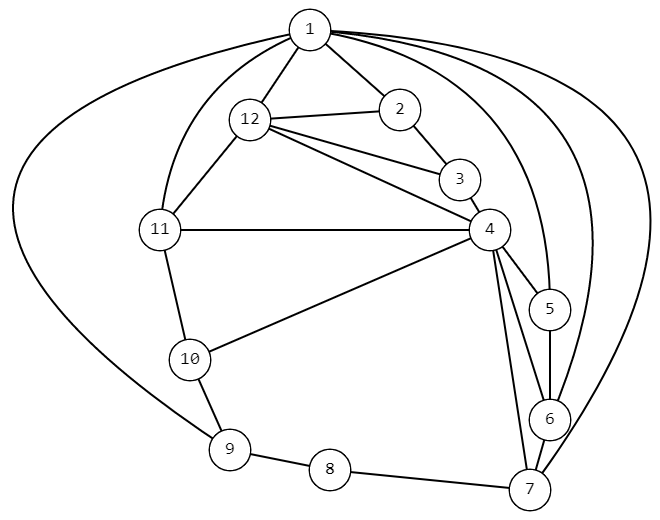
\includegraphics[scale=0.5]{graph.png}
\end{center}

Удалим из ψG ребра, которые вошли в ψ1 и ψ5.

$\psi_{1} = \{\}$

$\psi_{2} = \{u_{5\ 12}\}$

$\psi_{3} = \{u_{2\ 9}\}$

$\psi_{4} = \{u_{3\ 10}\}$

$\psi_{5} = \{\}$

$\psi_{6} = \{u_{5\ 12}\}$

$\psi_{7} = \{\}$

$\psi_{8} = \{\}$

$\psi_{9} = \{u_{2\ 9}\}$

$\psi_{10} = \{u_{3\ 10}\}$

$\psi_{11} = \{\}$

Удаляем ψ 1 ,  ψ 5 , ψ 7 , ψ 8 , ψ 11 так как они пусты и объединяем одинаковые семейства


$\psi_{2} = \{u_{5\ 12}\}$

$\psi_{3} = \{u_{2\ 9}\}$

$\psi_{4} = \{u_{3\ 10}\}$



% $\alpha_{23} = |\psi_{2}| + |\psi_{3}| - |\psi_{2} \cap \psi_{3}| = 1 + 1 - 0 = 2$

\begin{center}

  \begin{tabular}{|c|c|c|c|c|c|c|c|c|c|c|c|c|c|c|} \hline
       & 2 & 3 & 4  \nl
    2  & 0 & 2 & 2  \nl
    3  &   & 0 & 2  \nl
    4  &   &   & 0  \nl
  \end{tabular}
\end{center}

$max α_{γδ} = 2$, дают пары множеств: ψ 2 ψ 3, ψ 2 ψ 4, ψ 3 ψ 4 .

Возьмем множества

$\psi_{2} = \{u_{5\ 12}\}$

$\psi_{3} = \{u_{2\ 9}\}$

В суграфе H, содержащем максимальное число непересекающихся ребер,
ребра, вошедшие в ψ 2 , проводим внутри гамильтонова цикла, а в ψ 3 – вне
его.

\begin{center}
  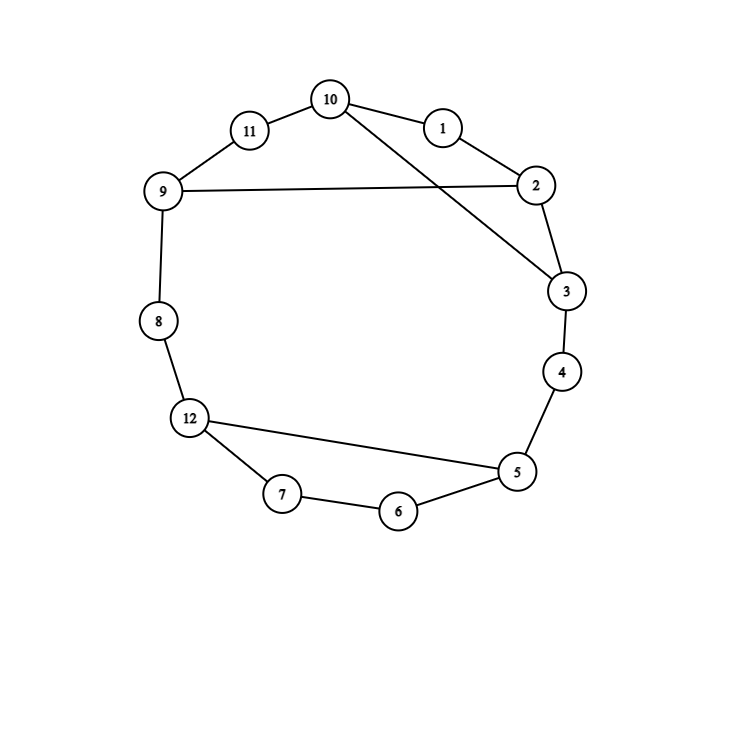
\includegraphics[scale=0.5]{graph2.png}
\end{center}

Удаляем из Ψ G’ ребра, вошедшие в ψ 2 , ψ 3

$\psi_{2} = \{\}$

$\psi_{3} = \{\}$

$\psi_{4} = \{u_{3\ 10}\}$

Объединяем одинаковые множества:

$\psi_{4} = \{u_{3\ 10}\}$

\begin{center}
  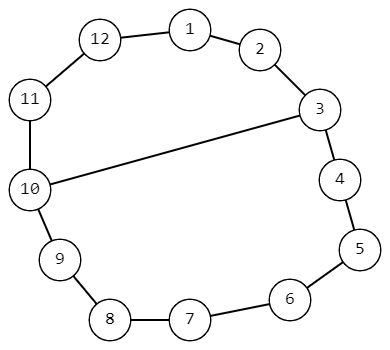
\includegraphics[scale=0.5]{graph3.png}
\end{center}

Удаляем из ΨG’ ребра, вошедшие в ψ4

$\psi_{4} = \{{}\}$


В Ψ G’ пусто – граф планаризирован.

При текущих условиях (при ограниченном количестве замененных ребер)
толщина графа m = 3. Если заменить все ребра – толщина будет другой.


\end{document}